\documentclass[a4paper]{article}
\usepackage[UTF8]{ctex}
\usepackage{geometry}
\usepackage{graphicx}
\usepackage{url}
\usepackage{multirow}
\usepackage{array}
\usepackage{booktabs}
\usepackage{url}
\usepackage{enumitem}
\usepackage{graphicx}
\usepackage{float}
\usepackage{amssymb}
\usepackage{amsmath}
\usepackage{subfig}
\usepackage{longtable}
\usepackage{pifont}
\usepackage{color}

\allowdisplaybreaks

\geometry{a4paper, scale=0.78}

% \begin{figure}[H]
%     \centering
%     \includegraphics[width=.55\textwidth]{E.png}
%     \caption{矩阵与列向量的乘法}
%     \label{fig:my_label_1}
% \end{figure}

% \left\{
% \begin{array}{ll}
%       x+2x+z=2 & \\
%       3x+8y+z=12 & \\
%       4y+z=2
% \end{array}
% \right.

% \begin{enumerate}[itemindent = 1em, itemsep = 0.4pt, parsep=0.5pt, topsep = 0.5pt]

% \end{enumerate}

%\stackrel{a}{\longrightarrow}

%\underbrace{}_{} %下括号

\title{Markov Chain Monte Carlo 06 Method of MCMC}
\author{Chen Gong}
\date{04 January 2020}

\begin{document}
\maketitle
这一小节主要是对前面的补充,希望可以详细的介绍一下MCMC原理,将前面的知识点可以顺利的串起来。MCMC采样中,我们借助了一条马氏链,马氏链的性质,经过若干步以后会收敛到一个平稳分布。马尔可夫链的组成可以大致分成两个部分:

1. 状态空间:$\{ 1,2,3,\cdots,k \}$;

2. 状态转移空间$Q=[Q_{ij}]_{k\times k}$。

马尔可夫链的模型可以被我们表达为:
\begin{figure}[H]
    \centering
    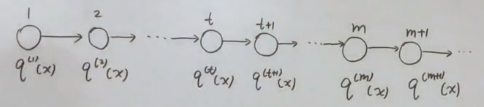
\includegraphics[width=.55\textwidth]{微信图片_20200103121212.png}
    \caption{马尔可夫链模型抽象图}
    \label{fig:my_label_1}
\end{figure}

每一个时间点有一个状态分布,表示当前时间点位于某个状态的概率分布情况,我们表示为$q^{(t)}(x)$。如果,是在$t=1$的时间节点,状态的概率分布为$q^{(1)}(x)$,我们可以用下列表来描述:
\begin{center}
\begin{tabular}{c|ccccc}
     $x$ & 1 & 2 & 3 & $\cdots$ & $k$  \\
     \hline
     $q^{(1)}(x)$& $q_1^1$ & $q_1^2$ & $q_1^3$ & $\cdots$ & $q_1^k$ \\
\end{tabular}    
\end{center}

我们假设在$t=m$时刻之后到达了平稳分布状态,那么我们就可以得到:$q^{(m)} = q^{(m+1)} = q^{(m+2)}$。这时的平稳分布就是我们想要的目标分布。相邻时间节点之间的状态转移矩阵为:
\begin{equation}
    Q =
    \begin{bmatrix}
        Q_{11} & Q_{12} & \cdots & Q_{1k} \\
        Q_{21} & Q_{22} & \cdots & Q_{2k} \\
        \vdots & \vdots & \ddots & \vdots \\
        Q_{k1} & Q_{k2} & \cdots & Q_{kk} \\
    \end{bmatrix}_{k\times k}
\end{equation}

状态转移矩阵描述的是,$Q_{ij} = Q(x^2=j|x^1=i)$。描述的是从一个状态转移到另外一个状态的概率。所以,状态转移矩阵的每一行$i$表示为目前状态是$i$时,到其他状态的概率,那么必然有$\sum_{k=1}^k Q_{ik} = 1$。实际上了解强化学习的同学,对于这些概率应该是非常的熟练了,这些都是强化学习的基础。

\section{Markov Chain 收敛性介绍}
在这一小节中,我们将详细的介绍一下,Markov Chain中状态转移的过程。并将证明在Markov Chain随着迭代一定会收敛到一个平稳分布。

\subsection{Markov Chain状态转移计算}
假设在$t+1$时刻,状态是$x=j$,那么它的分布为所有可能转移到这个状态的概率$i$乘以这个状态的分布$q^{(t)}(x=i)$,我们用公式表达就是:
\begin{equation}
    q^{(t+1)}(x=j) = \sum_{i=1}^k q^{(t)}(x=i) Q_{ij}
\end{equation}

那么,这仅仅是当$x=j$时概率,实际上在$t+1$时刻,可能出现的状态有k个,那么$q^{t+1}$的分布,就是将转移到各个状态的概率分别计算出来,也就是如下所示:
\begin{equation}
    q^{(t+1)} = 
    \begin{bmatrix}
        q^{(t+1)}(x=1) & q^{(t+1)}(x=2) & q^{(t+1)}(x=3) & \cdots & q^{(t+1)}(x=k)  
    \end{bmatrix}_{1\times k}
\end{equation}

而,
\begin{equation}
    q^{(t+1)}(x=j) = \sum_{i=1}^k q^{(t)}(x=i) Q_{ij}
\end{equation}

那么,$q^{(t+1)}$可以被我们表示为:
\begin{equation}
\begin{split}
    q^{(t+1)} = &
    \begin{bmatrix}
        \sum_{i=1}^k q^{(t)}(x=i) Q_{i1} & \sum_{i=1}^k q^{(t)}(x=i) Q_{i2} & \cdots & \sum_{i=1}^k q^{(t)}(x=i) Q_{ik}
    \end{bmatrix}_{1 \times k} \\
    = & q^{(t)}\cdot Q
\end{split}
\end{equation}

其中,$q^{(t)} = \begin{bmatrix} q^{(t)}(x=1) & q^{(t)}(x=2) & q^{(t)}(x=3) & \cdots & q^{(t)}(x=k) \end{bmatrix}_{1\times k}$。那么,通过这个递推公式,我们可以得到,$q^{(t+1)} = q^{(t)}Q = q^{(t-1)}Q^2 = \cdots = q^{(1)}Q^t $。通过上述的描述,详细大家都已经详细的了解了Markov Chain中,每个时刻点的状态的分布$q^{(t)}$的计算方法。既然我们知道了每个时间点的概率分布的计算方法,下一个问题就是我们怎么可以知道一定是收敛的呢?

\subsection{Markov Chain 收敛性}
由于$Q$是一个随机概率矩阵,那么我们可以得到,每个值都是小于1的,所以也必然有特征值的绝对值$\leq 1$。为什么呢?我们可以从特征值的几何意义上好好的想一想,特征值代表变换中方向不变的向量的变化尺度。随机矩阵的变化尺度必然是小于1的。所以,我们可以对概率转移矩阵做特征值分解,分解成对角矩阵:
\begin{equation}
    Q = A\Lambda A^{-1} \qquad \Lambda = 
    \begin{bmatrix}
     \lambda_1 & & & \\
     & \lambda_2 & & \\
     & & \ddots & \\
     & & & \lambda_k \\
    \end{bmatrix}
    ,\qquad |\lambda_i| \leq 1
    \qquad (i = 1, 2, \cdots, k)
\end{equation}

我们假设只有一个$\lambda_i= 1$,则:
\begin{equation}
    q^{(t+1)} = q^{(1)}(A\Lambda A^{-1})^t = q^{(1)}A\Lambda^t A^{-1} \\ 
\end{equation}

当$t\rightarrow \infty$时,必然有:
\begin{equation}
    \Lambda^t = 
    \begin{bmatrix}
     0 & & & \\
     & 1 & & \\
     & & \ddots & \\
     & & & 0 \\
    \end{bmatrix}
\end{equation}

我们可以假设存在足够大的$M$:
\begin{equation}
    s.t.\quad \Lambda^M = 
    \begin{bmatrix}
     0 & & & \\
     & 1 & & \\
     & & \ddots & \\
     & & & 0 \\
    \end{bmatrix}
\end{equation}

所以,
\begin{equation}
    \begin{split}
        q^{(m+1)} = & q^{(1)} A\Lambda^mA^{-1} \\
        q^{(m+2)} 
        = & q^{(m+1)} A\Lambda A^{-1} \\
        = & q^{(1)} A\Lambda^mA^{-1} A\Lambda A^{-1} \\
        = & q^{(1)} A\Lambda^{(m+1)}A^{-1} \\
        = & q^{(m+1)}
    \end{split}
\end{equation}

通过上述的证明,我们成功的证明了$q^{(m+2)} = q^{(m+1)}$。我们用数学的语言来表述一下,也就是当$t > m$时,$q^{(m+1)} = q^{(m+2)} = \cdots = q^{(\infty)}$。这就是平稳分布,我们成功的证明了Markov Chain经过足够大的步数$m$之后,一定会收敛到一个平稳分布。于是,这就启发了我们设计一个Markov Chain,收敛到我们想要采样的分布$p(x)$。那么。怎么我们才能让它收敛呢?实际上就是由状态转移矩阵$Q$所决定的。我们的核心问题就是设计一个合适的状态转移矩阵$Q$。

那么,我们要做的就是{\color{red} 设计一个MCMC,利用Markov Chain收敛到一个平稳分布$q(x)$,使得平稳分布$\approx$目标分布$p(x)$。}也就是当$m$足够大的时候,$q^{(m)}(x) = q^{(m+1)}(x) = q^{(m+2)}(x) = q(x)$。

那么,我们的Markov Chain解决了当维度很高的时候,$q(x) \approx p(x)$找不到的情况,在MCMC中不要显示的去找,而是构建一个Markov Chain去近似,跳过了直接去寻找的过程。

这里我们介绍一个概念,也就是从开始到收敛到$m$的这段时期被我们称为bum-in,中文翻译为燃烧期(个人觉得非常的难听,所以我从来不用中文的表述形式)。也有说法称这个时间$t$为Mix-time。当然也不是任何的分布都可以用MCMC来进行采样。但是它可以有效的避免我们去寻找$q(z)$。下面我们将描述一些用MCMC采样时遇到的困难的地方。

\section{Existing Problem}
1. 虽然,我们可以证明出MCMC最终可以收敛到一个平稳分布。但是并没有理论来判断Markov Chain是否进入了平稳分布,也就是不知道Markov Chain什么时候会收敛。

2. Mixing Time过长,这就是有高维所造成的,维度和维度之间的相关性太强了,$p(x)$太过于复杂了。理论上MCMC是可以收敛的,但是如果$m$如果实在是太大的话,我们基本就是认为它是不收敛的。实际上,现在有各种各样的MCMC算法的变种都是在想办法解决这个Mixing Time过长的问题。

3. 我们希望采到的样本之间的样本相互独立,也就是采到的样本之间的相关性越小越好。

这个有关于样本之间独立性的问题,大家可能不太好理解,这是实际在高维分布中我们采用MCMC来进行采样很有可能造成样本单一,相关性太强的问题。我们我们来举一个Mixture Gaussian Distribution的例子。下图所示是一个Mixture Gaussian Distribution的例子:
\begin{figure}[H]
    \centering
    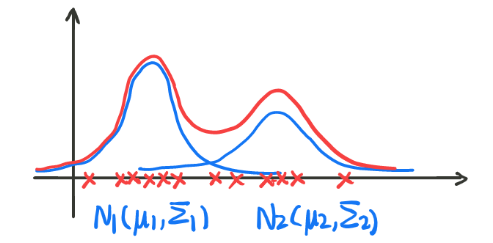
\includegraphics[width=.55\textwidth]{微信图片_20200103152759.png}
    \caption{Mixture Gaussian Distribution举例}
    \label{fig:my_label_1}
\end{figure}

会有一个什么问题呢?就是样本都趋向于一个峰值附近,很有可能会过不了低谷,导致样本都聚集在一个峰值附近。这个问题出现的原因我们可以从能量的角度来解释这个问题。在无向图中,我们常用下列公式来进行表示:
\begin{equation}
    P(X) = \frac{1}{Z} \hat{P}(X) = \frac{1}{Z}exp^{-\mathbb{E}(X)}
\end{equation}

实际上这里的$\mathbb{E}(X)$指的就是能量函数,能量和概率是成反比的,概率越大意味着能量越低,能量越低,越难发生跳跃的现象。所以,采样很容易陷入到一个峰值附近。并且,多峰还可以分为均匀和陡峭,陡峭的情况中,能量差实在是太大了,就很难发生跳跃。就像孙悟空翻出如来佛祖的五指山一样,佛祖的维度很好,孙悟空在翻跟头的时候,一直在一个低维里面不同的打转,根本就跳不出来,就是来自佛祖的降维打击。

所以,在高维情况下,很容易发生在一个峰值附近不停的采样,根本就跳不出来,导致采到的样本的多样性低,样本之间的关联性大,独立性低。

























\end{document}
